\documentclass{article}
\usepackage{amsmath}
\usepackage{amssymb}
\usepackage{tikz}
\usetikzlibrary{arrows}

\begin{document}

\section{Generalization Hierarchies for K-Anonymity}

\subsection{Age Domain Generalization Hierarchy (DGH$_{Age}$)}

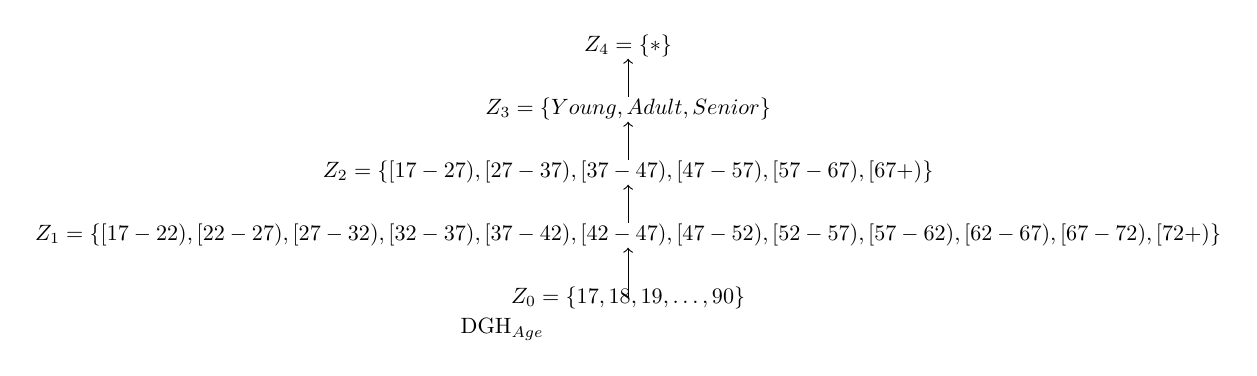
\begin{tikzpicture}[scale=0.8, every node/.style={transform shape}]
\node at (0,0) {$Z_0 = \{17, 18, 19, \ldots, 90\}$};
\node at (0,1) {$Z_1 = \{[17-22), [22-27), [27-32), [32-37), [37-42), [42-47), [47-52), [52-57), [57-62), [62-67), [67-72), [72+)\}$};
\node at (0,2) {$Z_2 = \{[17-27), [27-37), [37-47), [47-57), [57-67), [67+)\}$};
\node at (0,3) {$Z_3 = \{Young, Adult, Senior\}$};
\node at (0,4) {$Z_4 = \{*\}$};

\draw[->] (0,0) -- (0,0.8);
\draw[->] (0,1.2) -- (0,1.8);
\draw[->] (0,2.2) -- (0,2.8);
\draw[->] (0,3.2) -- (0,3.8);

\node at (-2,-0.5) {DGH$_{Age}$};
\end{tikzpicture}

\subsection{Education Domain Generalization Hierarchy (DGH$_{Education}$)}

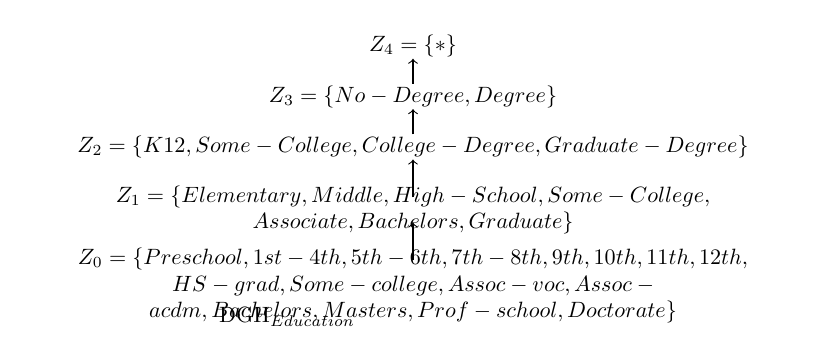
\begin{tikzpicture}[scale=0.8, every node/.style={transform shape}]
\node at (0,0) {\parbox{12cm}{\centering $Z_0 = \{Preschool, 1st-4th, 5th-6th, 7th-8th, 9th, 10th, 11th, 12th,$\\$HS-grad, Some-college, Assoc-voc, Assoc-acdm, Bachelors, Masters, Prof-school, Doctorate\}$}};
\node at (0,1.2) {\parbox{10cm}{\centering $Z_1 = \{Elementary, Middle, High-School, Some-College,$\\$Associate, Bachelors, Graduate\}$}};
\node at (0,2.2) {$Z_2 = \{K12, Some-College, College-Degree, Graduate-Degree\}$};
\node at (0,3) {$Z_3 = \{No-Degree, Degree\}$};
\node at (0,3.8) {$Z_4 = \{*\}$};

\draw[->] (0,0.4) -- (0,1.0);
\draw[->] (0,1.4) -- (0,2.0);
\draw[->] (0,2.4) -- (0,2.8);
\draw[->] (0,3.2) -- (0,3.6);

\node at (-2,-0.5) {DGH$_{Education}$};
\end{tikzpicture}

\subsection{Marital Status Domain Generalization Hierarchy (DGH$_{Marital}$)}

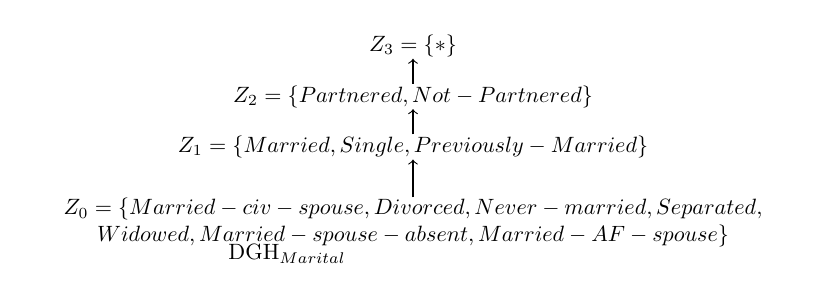
\begin{tikzpicture}[scale=0.8, every node/.style={transform shape}]
\node at (0,0) {\parbox{12cm}{\centering $Z_0 = \{Married-civ-spouse, Divorced, Never-married, Separated,$\\$Widowed, Married-spouse-absent, Married-AF-spouse\}$}};
\node at (0,1.2) {$Z_1 = \{Married, Single, Previously-Married\}$};
\node at (0,2) {$Z_2 = \{Partnered, Not-Partnered\}$};
\node at (0,2.8) {$Z_3 = \{*\}$};

\draw[->] (0,0.4) -- (0,1.0);
\draw[->] (0,1.4) -- (0,1.8);
\draw[->] (0,2.2) -- (0,2.6);

\node at (-2,-0.5) {DGH$_{Marital}$};
\end{tikzpicture}

\subsection{Race Domain Generalization Hierarchy (DGH$_{Race}$)}

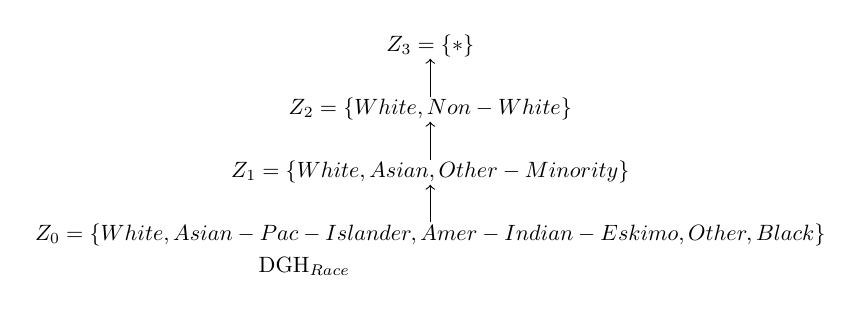
\begin{tikzpicture}[scale=0.8, every node/.style={transform shape}]
\node at (0,0) {$Z_0 = \{White, Asian-Pac-Islander, Amer-Indian-Eskimo, Other, Black\}$};
\node at (0,1) {$Z_1 = \{White, Asian, Other-Minority\}$};
\node at (0,2) {$Z_2 = \{White, Non-White\}$};
\node at (0,3) {$Z_3 = \{*\}$};

\draw[->] (0,0.2) -- (0,0.8);
\draw[->] (0,1.2) -- (0,1.8);
\draw[->] (0,2.2) -- (0,2.8);

\node at (-2,-0.5) {DGH$_{Race}$};
\end{tikzpicture}

\section{Hierarchy Specifications}

\subsection{Information Loss by Level}
\begin{align}
\text{Age: } & IL_1 = 0.2, \quad IL_2 = 0.4, \quad IL_3 = 0.7, \quad IL_4 = 1.0 \\
\text{Education: } & IL_1 = 0.15, \quad IL_2 = 0.35, \quad IL_3 = 0.65, \quad IL_4 = 1.0 \\
\text{Marital: } & IL_1 = 0.3, \quad IL_2 = 0.6, \quad IL_3 = 1.0 \\
\text{Race: } & IL_1 = 0.4, \quad IL_2 = 0.7, \quad IL_3 = 1.0
\end{align}

\subsection{Generalization Functions}
For each quasi-identifier $q_i$ and generalization level $l$:
$$gen(q_i, l): Domain(q_i) \rightarrow Z_l$$

Where $Z_l$ represents the generalized domain at level $l$.

\end{document}